\documentclass[12pt,a4paper]{article}
\usepackage[utf8]{inputenc}
\usepackage[english]{babel}
\usepackage{amsmath}
\usepackage{amsfonts}
\usepackage{amssymb}
\usepackage[left=2cm,right=2cm,top=2cm,bottom=2cm]{geometry}
\author{Adrian Bach}
\title{Using artificial intelligence to improve decision-making in conservation conflicts \\\medskip Ten-week report}

% bibliography 
\usepackage{natbib}
\bibliographystyle{humannat}

\begin{document}
\maketitle

%\newpage
\tableofcontents

\newpage
\section{Context}
\subsection{Conservation}

%6th mass extinction? Ref: \\
At the beginning of what could be a new mass extinction episode (LACKS REF), preserving the remaining "Nature" is a central concern for humanity, as it undeniably depend on the services ecosystems provide. (no need for references, right?)
Pollination, soil enrichment, water treatment, carbon dioxide fixation, among many more, are essential for human survival (REF) and the role of nature in human well-being is increasingly recognized (REF).
However, the key for the permanence of ecosystems is diversity, as it ensures a quick and dynamic response to change(REF).
Note that this variety is often an inspiration for innovation in any kind of technology.
Thus, conservation of biodiversity have become a leading field in ecology.
%
%One of the many aspects, intense competition/antagonism between human activity and wildlife. Ref: \\
%Conservation as a way to tame this problem. Ref: \\
%
%\subsection{Conservation}

According to ... Definition of conservation.\\
%Different kinds of conservation actions.
Conservation can be applied in many different ways.
It can be preventive, by establishing protected areas to preserve intact ecosystems from human impact \citep{vanwilgen2011critical, bainbridge2017goose}, or to restore already damage ecosystems \citep{rumpff2011state}. 
%: protection areas, ?. Ref: Wilgen2011, Brainbridge2017.
It can also be in reaction to a ongoing problem without preventing contact, \textit{e.g.} culling control by monetary incentives \citep{mason2017changing, cusack2018time}.
Another example is offsetting, which is balancing "local habitat destruction by restoring, enhancing and/or protecting similar but separate habitat" \citep{gordon2011assessing}.
%But conserving a species for its own sakes sometimes lead it to reach numbers being problematic for human activities. Ref: Redpath's book.
There are many other examples, but genuinely successful implementation of conservation is scarce because of the numerous challenges it faces \citep{keith2011uncertainty, vanwilgen2011critical}.\\
%
%\subsection{Problems faced}

%\subsubsection{Complexity}
Conservation problems are recognized as highly complex and densely interconnected systems, including ecology, sociology, agronomy and climatology simultaneously.
Indeed, socio-ecosystems exhibit most of the characteristics \cite{game2013conservation} attributes to complex systems: "numerous interacting elements lacking any central control, non-linear interactions between elements, constant change which is seldom reversible, and no clearly defined boundaries".

%It makes their complete understanding out of our cognition.
%Ref: grimm1999individual, wilgen2011critical, runge2011uncertainty, schluter2013new,pretty much every article I've read.
In such systems, it is often impossible to isolate a causes of the changes.
%\subsubsection{Lack of data}
The response to a conservation action is lost in other signals from a myriad of uncontrollable external factors.
Thus, monitoring the system's response to a policy over time can be very expensive, time demanding, and often irrelevant, as the number of possible variables is too large.
Thus, conservation policies often lack data to account for their effectiveness, or to understand failure \citep{keith2011uncertainty}.
Furthermore, management is based on estimations of populations, which accuracy varies according to the technique \citep{BUNNEFELD2011441}.
%Ref: rumff2011, all of the articles from the 2011 special edition.

%\subsubsection{Rigidity}
Due to its complexity, predicting the system's response to a change in the conservation policy is very challenging.
It can results in reluctance to change, and in the maintain of inadequate conservation policies \citep{keith2011uncertainty, peterson2005conservation}.
%Ref: geese case, apply a simple protection lead to population reaching conflictual numbers.
Broadly speaking, conservation faces uncertainty at many levels.

%Other limits in keith2011uncertainty about politics and self-serving.
Moreover, conservation often takes place in a political context, and can be significantly slowed, even blocked, by indifferent politics or lobbies for interests that would not benefit from conservation policies \citep{keith2011uncertainty}.
Unexpectedly but fortunately, there is little evidence that bigger budgets make conservation easier or more effective \citep{game2013conservation}.

%Conservation had to be carried on despite these potentially discouraging barriers, acting on protection while dealing with them.
So how to conduct efficient conservation, while dealing with these discouraging barriers and embracing uncertainty?

\subsection{Adaptive management}
%
%\subsection{Purpose}

%how it deals with certain problems. Acting while acquiring informations, learning from mistakes, closer to the system response to act as quickly as possible.
Adaptive Management (AM) suggests to dynamically update the management policy according to the system's behaviour.
This way, conservation can be better fitted to the system, and acting regularly allow to acquire informations on its response to change.
Therefore, managers can learn heuristically from the system, and react effectively.
%Uncertainty is an irreducible aspect of conservation, so it seems more relevant to act embracing it rather than waiting and keep on with an inadequate policy.
And although AM also relies on the monitoring of some selected variables, their choice can adapt dynamically to the problems detected after each policy updating.
LACKS REF\\
%
%\subsection{Limits}
%
%critics from game2013.\\
Yet, \cite{game2013conservation} argues that implementing any new decision will result in a complex change in the system, and that as soon as it has changed it is not comparable to its previous state any more.
This artefact can be reduced in small-scale, simpler systems, to which AM would then be particularly adapted.
%
%other unresolved problems from above.
%Even if AM represent one of the most efficient way to deal with uncertainty in conservation, it is still facing politic-related opposition.

A major concern in current conservation is that, even if a policy effectively protects a species from going extinct, mismanagement can lead populations to reach problematical numbers for human livelihood.

\subsection{Conflicts}

This is when conflicts arise, because people impacted by a protected population's growth are very likely to defect conservation policies, which can be threatening for the species persistence.
Definition of a conflict. Ref: Redpath's book.\\
ConFooBio is a gathering of well monitored cases of conservation conflicts (see figure \ref{confoobio}).
There are some more examples in (Redpath's book, redpath2013) with leopards etc. YET TO FILL
%mason2017.
and in \cite{behr2017combining} with wolves and livestock in the french Alps.
%, or Rhinos conservation and illegal poaching for Ivory in south Africa \citep{glynatsi2018evolutionary}.
%Resolving these conflicts requires effective management strategies.
%Management strategy: a sequence of actions on the system in order to achieve goals.\\
%Yet, ecosystems dynamics are highly complex and interconnected, their evolution very difficult to anticipate.

%\subsection{Divergent interests between stakeholders}
In these conflicts, the divergence of stakeholders interests makes conservation even more complicated.
Yet, meeting every stakeholder interests is the only way for a management policy to be sustainable, because defection is less likely.
Indeed, farmers are usually way more interested in the yield they live on, then in the survival of the species that is part of its decreasing.
Reaching a consensus on a target for the population can therefore be an unproductive process.
Moreover, it can prevent the situation from changing in a more equitable way \citep{peterson2005conservation}.\\
%
%\subsection{MSE}

Management Strategy Evaluation is a framework that describes the process of Adaptive Management in conflictual situations.
It decomposes the problem in four main parts: manager's policy updating, user's harvest strategy, the species population and the mode of estimation of the population (see figure \ref{msediagram}). ADD FIGURE
This structure isolates uncertainty at four main levels: decision-making under uncertainty, the reaction of the users, the population's response,
%links between components of the ecosystems,
and its estimation.
%politics
%All the problems it deals with.
The circular structure is adapted to the heuristic updating of management policy.
Putting manager and user into different parts recognizes different interests and expectations for conservation, and describing goal-oriented behaviours, unlike consensus-based policies.
It was successfully implemented in fisheries at first, and than applied on terrestrial animals conservation \citep{BUNNEFELD2011441, bunnefeld2013incentivizing}.
%Still need to establish targets.

\subsection{Modelling}

Since an accurate prediction of these socio-ecosystems' response is hardly possible, any conservation frameworks benefits from a modelling approach.
Conceptual models allow for the rapid exploration of different scenarios under certain hypotheses, thus being very useful decision-helping tools.
%
%\subsection{Different models used in literature}

%Ref: schluter2012, rumpff2011 (dealt with uncertainty by implementing different scenarios), bainbridge2017.
For example, \cite{rumpff2011state} used a Bayesian network to model the transitions between the possible state of a landscape according to a policy, to plan for the restoration of different protected areas previously damaged by human activity.
The book from \cite{schluter2012new} threw the stones of socio-ecological modelling in order to manage conservation involving human compliance (an extensive list of studies using modelling in conservation is presented in chapter 2.1).
The high diversity of models also highlights the lack of common framework, to which MSE is a strong candidate.
In the conclusion, the authors stated that a proper modelling framework for conservation conflicts needs human decision-making modelling, because unforeseen non-compliance was one of the main causes for failures.\\
%
%\section{Decision-making modelling}

Game Theory (GT), introduced by John Von Neumann and Oskar Morgenstern in 1944 in the book "The Theory of Games and Economic Behavior", is commonly recognized as the leading framework for decision-making modelling.

%\subsection{Game theory}
\cite{myerson1997game} describes GT as follows: "\textit{the study of mathematical models of conflict and cooperation between intelligent rational decision makers [which choices] affect one another welfare}".
\textit{Games} are simplified vision of actual conflicts, their actual complexity being unreachable.
But such complexity prevents from understanding the fundamental issues of conflict and cooperation.
As any other scientific work, game models deliberately omit less relevant details of actual situation to allow the study of particular phenomenon in the scope of a particular question.
In these games, players act in order to maximise the expected value of the game's outcome, the so-called \textit{utility}.
Utility is not necessarily quantified as monetary pay-off, it can be seen in many different ways (time, effort saved, well-being, happiness, ..) and even a mix of them.
Game theoretical perspective can provide insights about: "the strategies different stakeholders will likely adopt given their objectives, [\dots] the range of possible outcomes, [\dots] and whether an optimal or satisfactory solution for all stakeholders can be reached simultaneously" \citep{COLYVAN20111246}.
It was first used in Biology in \cite{maynard1973logic} to investigate the evolution of animal strategies in con-specific fights.
%Definition of the key concepts like utility. Ref: myerson1997.

%\subsection{Application to conservation conflicts}
\cite{COLYVAN20111246} investigated theoretical applications of the four main types of games (simple, chicken, stag and prisoner games) to Adaptive Management, but its actual implementation for conservation purposes is fairly novel. 
\cite{glynatsi2018evolutionary} modelled the existing conflict between rhinos protection and illegal poaching for ivory as a common-pool resource problem, to assess which proportion of rhinos should be de-horned to minimize their killing, according to poacher being unconditional or selective killers.\\ %(figure \ref{rhino-poachers-game}).
%\begin{figure}
%	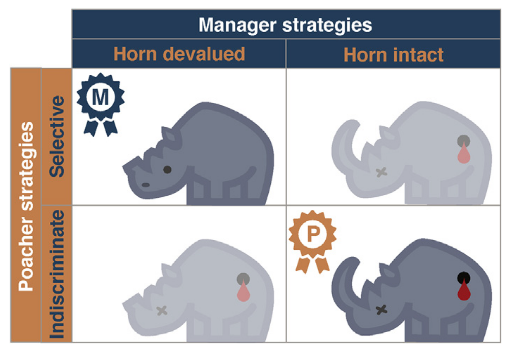
\includegraphics[scale=0.5]{rhinos-poachers-game.png}
%	\caption{The game between rhino manager and rhino poachers. The system settles to one of two equilibriums, either devaluing is eff ective or not. N.E. Glynatsi et al.}
%\end{figure}
Recently, a model developed on MSE framework, including decision-making modelling within Game Theory, was introduced in \cite{duthie2018} .

\section{GMSE}%Ref: duthie2018gmse. emphasize on its novelty.

\subsection{Formalisation of MSE framework}

%describe how it falls in MSE framework, how it deals with uncertainty at each level, consensus biases, long term foreseeing.
%At four main levels: population dynamics, links between components of the ecosystems, type of estimation of the population, making the right decision without knowing precisely the outcomes, reaction of the users, politics, response of the system, ...\\
%Explain clearly what it is meant for.
GMSE is a mathematical formalisation of MSE framework, assigning each part a conceptual model.
It aims at exploring the long-term consequence of a given management strategy, in order to test its effectiveness, and highlight potential problems managers would not have thought of.\\
According to MSE framework, a policy is effective when, after the chosen period of management:
\begin{itemize}
    \item The population (i) does not go extinct and (ii) stabilizes around the conservation target.
    \item The users' yield reaches a satisfactory percentage.
    \item All users have comparable yield percentages.
    \item The spatial distribution of the resource is equitable between users' lands.
\end{itemize}
If these condition are fulfilled, there should not be any reason left for conflict to persist.
GMSE can be used both for investigation \citep{cusack2018time}, and application to conservation \citep{bainbridge2017goose}.\\

Concerning the mathematical formalisation, the population changes at each time step according to a spatially explicit, individual-based population dynamic model.
Each individual is born, moves, and dies according to probabilities drawn in defined laws to account for the uncertainty on population dynamics.\\
The population is monitored according to different definable techniques, some of which includes probabilities of detection, thus accounting for the uncertainty about the accuracy of monitoring.\\
The manager model can be parametrized to reflect its conservation goals.
It uses the information from the monitoring to set a policy.
A policy is a set of possible actions associated with a cost for its performance.
The manager has a given budget, and implementing a policy implies a cost for him/her.\\
The user model is individual-based, and each user can be parametrized to reflect its aims concerning the population.
There can be several users, and they are modelled independently.
Each has a given budget, and acts according to the number of actions she/he can perform according to their cost set by the manager, in order to achieve his/her goal (figure \ref{gmse-diagram}). ADD FIGURE\\
%\subsection{First IBM in conservation}
%
%"Individualbased
%models (IBMs; also known as agent-based models) are
%used to model the behaviour of a system at an individual level
%by specifying simple rules for agents and allowing them to
%interact. These models allow for complex behaviour to emerge
%from simple interactions, though this comes at some cost to
%interpretation and analysis." Ref: hamblin2012parctical.

\subsection{Decision-making artificial intelligence}

%Genetic algorithm. Very accessible worded explanation. ref: hamblin2012practical\\
%How is it suited to human decision-making?\\
%Also used in solving game theoretical problems. Ref: Maynard Smith 1982.\\\
%An example of interaction between IBM and genetic algorithm was in hamblin2009, where the parameter governing the interaction rules in foraging ants where allowed to evolve through a GA.
The manager's and the users' decision are made by calling a Genetic Algorithm.
In the first place, GA were used to model the evolution of genes frequency in a population under stochastic recombination and mutation.
It has previously been used in combination with an individual-based model in a ant collective foraging model.
The parameter governing the interaction rules was allowed to evolve according to a GA.
Although this algorithm was not exactly successful in mimicking evolution, it inspired a new kind of Artificial Intelligence \citep{hamblin2013practical}.\\
In GMSE, a population of random strategies (an list of costs associated to actions) of a given size is initiated, and then allowed to evolve through stochastic mutation and crossing-over.
Each strategy's fitness to the decision-maker criteria is assessed, and the fittest are allowed to reproduce.
The process is repeated until the increase in fitness between the current fittest and the previous one falls under a given threshold.\\
It is particularly well fitted to human decision-making in this context, because due to the complexity of the problem, the decision-maker does not know in advance the best choice, but can judge if a choice is better than another.
Furthermore, humans are usually not able to explore all the possibilities to choose the best one, they select the best among the one they could think of.
%
%\subsection{Some limits to explore}
%
%\subsubsection{Theoretical}

%Agents act independently, which is very unlikely. REF???!!\\
In GMSE current version, the users act independently, regardless of their neighbours' behaviour.
This is very unlikely, as seen in the role-play games performed in \cite{redpath2018games}.
Also, Game Theory explicitly showed how crucial was the ability to know the other players' strategy to get the most out of the game's outcome.
%Different types of conservation interests.
Besides, at the moment, the manager's only goal is to maintain the population, but \cite{holmes2017understanding} showed that the interests of conservationists can be broader and more complex.
%Would be interesting to implement.\\
%Does not consider the do nothing option which is sometimes interesting.\\
Another feature that could be explored is the frequency of policy updating, currently quite rigid, as the manager acts whenever she/he is meant to, regardless of the situation.

%\subsubsection{Computational}
On the computational side, computing time increases greatly with the number of stakeholders, due to the individual-based approach.
%Lacks machine learning to be a proper artificial intelligence.
Furthermore, it is now complicated to speak about AI without including Machine Learning, yet Genetic Algorithm is not a structure that can be trained.

\section{Research Questions}
%They have to be very closely related to conservation (to avoid making it a mere modelling project)

\subsection{Case study: Geese}

I will focus on an actual case study of conservation conflict to keep GMSE development into a down-to-earth situation, and parametrize simulations with actual measures from the field.
I chose the case of conflict between geese population and farming on the Isle of Islay (Scotland) as it is a well documented case, with very accessible data within the team.

%Description. Ref: mason2017, brainbridge2017.
Geese endangered status was recognised during the 1940's, and was caused by "a combination of hunting for food and sport, systematic persecution and the disruption of the Second World War".
Protection measures were really efficient as, in the 1980's, all geese species population numbers increased significantly.
But this rise in population started a conflicts with farmers, as geese were intensely grazing their crops.
Especially for farmers owning culture in Special Protection Areas required by the European Bird Collective.
The first arrangements between the state and these farmers concerning geese control were made in the early 1990's, in the form of payments from government for farmers to allow undisturbed grazing on certain areas, and scare them away in others areas.
Yet, some populations are still increasing nowadays, and farmers started to consider the financial compensation too low for the damages caused.
But Scottish government refused to increase them for financial reasons.
Farmers then started to control the population by means unapproved by the conservation scheme \citep{bainbridge2017goose}.

%Its attributes (liked with the limits of GMSE).
This case is particularly adapted to work on the limits of GMSE.
It is a small scale case of conservation conflict, involving a handleable number of neighbouring users, that are very likely to interact in different interesting ways.
It is already a case of interest for Scottish National Heritage, and part of ConFooBio project, so the goose population, along with the updates in the conservation policy, have been regularly monitored for years.
Furthermore, this situation could clearly benefit from the results of this project, and could be an interesting way to test the applicability of GMSE to actual cases once again.
%from now on always speak about goose, state and farmers to settle the problem in the context of geese

\subsection{How does flexibility in policy updating frequency affect geese management strategy efficiency?}
%\subsubsection{Action threshold}
%%Currently in GMSE, a parameter sets the number of the manager's interventions per time step. Rigid, insensible to the situation, action if pop $>$ ou $<$ target, regardless of the size of this difference. acting even if the population if only a few individuals from the target.\\
%First, fixed deviation from manager's target as an action threshold. has to be relative the the population size though, if population size is 100, 50 individuals missing or extra is very concerning, yet it is less if population size is tens of thousands. For example I could test thresholds of 1, 5, 10, \dots \% of target.\\ 
%Quantitative assessment of the impact on the "quality" of the policy over repeated simulations for increasing threshold values: mean deviation from manager's target? Impact? Conflict reduction? number of extinctions? (Is there a chance that the result will be the same as the manager intervention frequency?)\\
%Dynamic threshold? A function of deviation from target, or conflict intensity, that would modify the action threshold.\\
%Waiting could imply saving a certain amount of budget for next step. Something that could also concern the users, maybe highlighting a best time to act.
%Recently introduced in iacona2017evolutionary: optimal delay before using funds.
Optimal growth in finances, or plant, sometimes included doing nothing, more precisely to invest less resources than usual in buying (balancing consumption and capital investment) or reproduction (less investment in seeds or flowers and more in root stock or growth, waiting for a less unsuitable or competitive time) for a certain amount of time.
Since the problems conservation is dealing with are often irreversible, managers are used to invest financial resources in acting as soon as they get them.
%Optimal growth concept applied to management strategy shows that investing in other domains than policy application is sometimes more profitable for conservation goals, if the possible outcome outweigh the increase in threat in the meantime.
%By doing nothing, authors mean invest in other domains than policy application, such as research, monitoring, or even other lucrative placements.
%But only if the possible outcome outweigh the increase in threat in the meantime.\\
Indeed, the complexity of conservation problems results in temporal heterogeneity.
Therefore, acting can be more efficient at certain moments than others, if the possible outcome outweigh the increase in threat to the protected species in the meantime.
%Just as conservation outcomes can be improved by "identifying the most efficient locations to act in space",
Thus, finding the best time to act could lead to more efficient management strategies \citep{Iacona2017waiting}.
%
%%\subsubsection{Calculus of impact}
%In \cite{gordon2011assessing}, the efficiency of offsetting is assessed by the "impact" of the policy implementation.
%It is the difference in the amount of native habitat loss when offsetting or not.
%This could be a interesting condition to assess whether manager should update the policy at this time or not. PAS A LA BONNE PLACE

Currently in GMSE, a parameter sets the number of the manager's interventions per time step.
And according to \cite{duthie2018}, the number of extinctions over several simulations of GMSE decreases exponentially with increasing frequency of manager intervention.
%So, I suspect it is going to show that doing nothing is not sustainable as a policy in itself. Surprise!
But does it means acting as soon as possible is an efficient strategy?
%I will answer this question by implementing new features in GMSE, and assess the efficiency of management strategies using them.

To answer this, I will implement a 'doing nothing' option in GMSE, as a bypass of policy updating under certain conditions at a given time step.
The most intuitive one would be the deviation of estimated population from the manager's target.
For now, the manager updates the policy whenever he/she is meant to, even if the estimated population is only a few individuals away from the target.
To loosen this condition, I will implement an action threshold $A$ based on $D$, the ratio of estimated population to manager's target.
If at this time step, $|1 - D| < A$, the policy will not be updated, meaning that the manager would act only if the population exceeds or goes under its target by a certain value set by $A$.

First, $A$ will have a fixed value along the conservation scheme period.
To quantitatively assess the effect of this strategy on management efficiency, I will select a set of relevant values for $A$ and run multiple simulations for each of them (probably a hundred replicates per $A$ values).
For each $A$ value, I will gather different informations from the simulations, according to the MSE criteria for an efficient management strategy.
\begin{itemize}
	\item The number of simulations in which the geese population went extinct, divided by the number of replicates, to estimate a probability of extinction.
	\item The mean deviation of the actual geese population from conservation target over the conservation scheme period, and average it over all the replicates.
	\item The mean total crop yield percentage across the conservation scheme period, averaged over all the replicates.
	\item The variability in crop yield percentage across the different users, averaged over all the replicates.
	\item The mean variability in the number of individuals per land unit across the different users, averaged over all the replicates.
\end{itemize}
I will use these measures to compare the effectiveness of the management strategy according to the value of $A$, and eventually highlight the most efficient one.

I have also thought of another way to find an optimal value for $A$, involving a more dynamic way to set it during the conservation scheme period.
The value of $A$ could be a Gaussian or a stair function of a variable describing the situation ($|1-D|$ for example, see figure \ref{dynamicA}), centred on a maximum value for $A$.
That way, if the situation is concerning at this time step, it could mean that the previous $A$ value was too high, thus the manager can adjust it to react more sensibly from now on.
I will run multiple replicates for different parameters values for the link-function between $A$ and the variable describing the situation.
From the simulation output, I will assess the evolution of the mean $A$ value over the replicates at each time step, along the conservation scheme period.
This will eventually show the emergence of an optimal value for the action threshold according to the link-function shape and parameters.

Finally, an interesting feature to add to this exploration would be the ability for the manager to save some budget for next time step if she/he decided not to act this time step.
I could assess the efficiency of the policy according to different percentages of budget saving, with the same method as previously.
%According to \cite{duthie2018}, the number of extinctions over several simulations decreases exponentially with increasing frequency of manager intervention. %So, I suspect it is going to show that doing nothing is not sustainable as a policy in itself. Surprise!
%But does it means acting as soon as possible is is a sustainable strategy?

%
%\subsection{Including human values in adaptive management}
%
%All conservationists have different goals according to their values, it would be interesting to implement this. Using the framework from futureconservation.org, I could use quantitative measures of conservationists values and attribute utilities accordingly, and assess if it indeed produce the expected results. Users yields and population size according to the value on nature - people axis, and to conservation - capitalism one. 

\subsection{How to manage geese population efficiently taking into account interactions between stakeholders?}

The main research goal of this project is to allow the decision-making AI to consider interactions between agents.
For example, in GMSE current version, the users act independently, regardless of their neighbours' behaviour.
This is very unlikely, as seen in the role-play games performed in \cite{redpath2018games}.
Also, Game Theory explicitly showed how crucial was the ability to know the other players' strategy to get the most out of the game's outcome.
I will take advantage of the first research question to get familiar with the case study, as well as GMSE code, in order to find out what kind of interactions are at play here, and how to implement them within the existing structure of the software.
After that, I will be able to assess how it affects the way managers make policies.
This is a real challenge because, to my knowledge, it has not been explored before.

\subsection{Next challenges}

GMSE being a completely novel software, there are still many ways to keep on developing it.

%\subsubsection{Computational}
From a computational point of view, computing time increases greatly with the number of stakeholders, due to the individual-based approach crossed with the systematic calling of the Genetic Algorithm.
This could be improve using parallel computing.
With the adapted software and code language, this technique allows to make many similar tasks simultaneously instead of in sequentially, thus highly increasing the throughput (number of operations per time unit).

Furthermore, it is now complicated to speak about AI without including Machine Learning, yet Genetic Algorithm is not a structure that can be trained.
To turn the decision-making AI into a learning structure, the team thought about a Neural Network (NN) in the shape of a map.
Given a variety of inputs, the NN would be able to output a land-use decision map.
The NN would be trained with data from numerous behavioural games performed within the ConFooBio project.
Once coded, this new version of GMSE could be compared to the previous one in terms of ability to manage conservation conflicts.
%\section{Expected outputs}
%
%At least a paper on the action threshold, a talk in Newcastle, a poster in winter symposium, a participation at the Trondheim workshop. Updated version of GMSE. Field work for SNH, possibly in the policy team to which Aileen is close.

\newpage
\bibliography{10WRbib}
\nocite{*}

\end{document}